\documentclass[12pt]{article}
\usepackage{mathptmx} % Use times new roman
\usepackage{geometry} % Sets paper type and margins
\geometry{letterpaper, margin=1in} 
\usepackage{graphicx} % Allows for imbedded images
\graphicspath{{media/}}
\usepackage{amsmath} % allows for imbedded equations
\usepackage{xfrac}

\title{ECEN 4610 -- Capstone Laboratory}
\newcommand{\subtitle}{Electrical Impedance Tomography Machine Design: An Open-Source Approach}
\newcommand{\department}{Department of ECE, University of Colorado, Boulder}
\newcommand{\location}{Grand Junction, CO, USA}
\author{Diego Sena, Jonathan Kleppinger, Keegan Erickson}
\date{\today}

\makeatletter
\def\@maketitle{% 
    \vspace*{\fill}
    \begin{center}%
        \let \footnote \thanks
        {\Large \@title \par}%
        \vskip 1em%
        {\LARGE \subtitle \par}%
        \vskip 1em%
        {\large \@date}%
        \vskip 1em%
        {\large
        \lineskip .5em%
        \begin{tabular}[t]{c}%
            \@author
        \end{tabular}\par}%
        \vskip 1em%
        {\large \department}%
        \vskip 1em%
        {\large \location}%
    \end{center}%
    \par
    \vspace*{\fill}}
\makeatother


\begin{document}
\begin{titlepage}
    \pagenumbering{gobble}
    \maketitle
\end{titlepage}

\tableofcontents
\pagebreak
\pagenumbering{arabic}
\section{Executive Summary}\label{executive-summary}
Electrical Impedance Tomography (EIT) is a non-intrusive medical imaging
technique for viewing a cross section of an area {[}1{]}. Common imaging
applications include the viewing of the heart and lungs, brain, and
breast tissue. Two currents 180 degrees out of phase into a plane of the
human body. Electrodes surrounding the cross-sectional area of the body
are used to measure varying voltages to create an image showing the
varying impedance, conductivity, and permittivity throughout the tissue
plane. This document outlines the design of an EIT machine using
programs and hardware aimed at creating cheaper and more open-source
methods of manufacturing, that are accessible to the general public and
university students.

\section{Problem Definition}\label{problem-definition}

\subsection{PROBLEM SCOPE}\label{problem-scope}

This paper documents the design and construction of an EIT machine using
methods and hardware that are accessible to the general public and
university students. The project sponsor for whom the development of the
EIT machine is being done is Dr. Talles Santos, a professor of
electrical engineering who is working for the University of Colorado,
Boulder.\\

The project sponsor has extensive experience in high quality EIT machine
development and research. Motivated by a desire to continue the research
in EIT and make the technology more accessible, the project sponsor
would like to use continued development of EIT to educate students in
the application of the technology. The project sponsor has experience
working with other grad students and professors on the development and
construction of EIT machines and would like to expand its development to
include the work of under grad students. Currently there is no EIT
machine at the location of Colorado Mesa University (CMU), where the
project sponsor is physically located and works. This project will be
the beginning of a goal to make CMU a new center for the development of
the technology.\\
The project sponsor has tasked the 2022-20123 senior design team with
starting a path to creating a fully open-source model for the
construction of an EIT machine. Using components available and
relatively inexpensive integrated circuit (IC) components, a fully
functional EIT machine with real-time imaging is to be constructed.~The
construction of the EIT machine was to maintain a cost below \$3,000.00
of the total budget.

\subsection{TECHNICAL REVIEW}\label{technical-review}

\subsubsection{INDUSTRY BACKGROUND}\label{industry-background}
Electrical Impedance Tomography (EIT) is a noninvasive medical imaging
technique. The imaging technique uses alternating current (AC) that is
injected into the human body to create a tomographic image of a cross
sectional area. Voltages are read through electrodes placed on the
surface of the skin surrounding the area to be imaged. The voltage
readings are then used along with the injection current to calculate
variations in impedance, conductivity, and permittivity through the
biological tissue to create the tomographic image of the cross-sectional
area.

Direct Current (DC) and low frequency electricity does not pass easily
through biological tissue. Which is the reason why higher frequency AC
electricity is needed. There is significant variation in impedance,
conductivity, and permittivity between different types of biological
tissue. This variation in impedance is what allows for the production of
tomographic images of the body. Variation in impedance is due to the
free ion content of tissue. Electrical impedance is shown by the
expression in Equation (1) {[}2{]}.

\begin{align}
    Z = R + jX
\end{align}

Where Z, the electrical impedance, is equivalent to R, the resistance,
and X the reactance. Conductivity and permittivity are typically what is
used in the actual imaging of tissue. Conductivity is the reciprocal of
impedance and is expressed in Siemens per meter (S/m). Typically, the
more fluid filled tissue is, the more conductive it is. Typical values
for conductivity are shown below in Table 1.~A specific organ of note,
the lungs, has much higher impedances than other organs. This is because
air has a very high impedance.

\begin{table}[h]
    \centering
    \caption{Shows the difference in conductivity between different tissue types{[}1{]}}
    \label{Table 1}
    \begin{tabular}{|l|l|}
    \hline
    \textbf{Tissue}     & \textbf{Conductivity ($\sfrac{mS}{m}$)} \\ \hline
    Cerebrospinal Fluid & 1450-1800                               \\ \hline
    Blood               & 500-650                                 \\ \hline
    Scalp               & 300-420                                 \\ \hline
    Brain               & 300-400                                 \\ \hline
    Muscle              & 200-400                                 \\ \hline
    Fat                 & 50                                      \\ \hline
    Bone                & 6                                       \\ \hline
    \end{tabular}
    
\end{table}

The differences in conductivity are mapped out using electrical
excitation caused by two injection current sources. These two injection
currents have the same frequency and amplitude but are 180° out of phase
from each other. While one injection current is positively charged, the
other will be negatively charged. In conventional current terms, current
will flow from positive charge to negative charge. Electrodes
surrounding the tissue are used during the current injection process to
take voltage readings. Current injection sites are at the same locations
as the electrodes, but only 2 at a time are activated at once. The
turned-on current injectors rotate to the next injectors after a period
of time that is optimal for the measurement process. The current
injectors that are turned on depend on the process chosen. Figure (2)
shows a visualization of the injected currents streamlines traveling
between the two current injection sources.

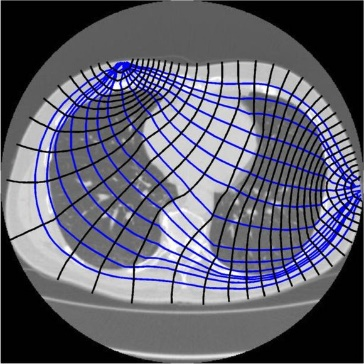
\includegraphics{media/image3.jpeg}

\subsubsection{CLIENT BACKGROUND}\label{client-background}

Dr. Talles Santos received his Bachelor of Science degree in electrical
engineering from the federal University of Minas Gerais, Belo Horizonte,
Brazil, in 2012, Earned a master\textquotesingle s degree in 2015 and
his PhD in 2019, both in control engineering and mechanical automation
from the Polytechnic School at the University of São Paulo, Brazil.

Dr. Santos has more than 10 years of experience in the EIT field. He
worked part time at Timpel Medical, São Paulo, Brazil, working on EIT
development {[}3{]}. Also, he has worked with several other groups
developing EIT for medical applications. Currently he is a professor of
electrical engineering who is working for the University of Colorado,
Boulder. He now wants to start further development of EIT technology at
CMU, while using the opportunity to educate students in the principles
of how EIT works and how to construct a machine. Dr. Santos wants to
make the technology cheaper and more accessible to medical professionals
and individuals who want to study and help further develop the
technology {[}3{]}. EIT machines require the coordination of high
frequency current injection, sampling processes, and control circuitry
at high speeds in order to achieve real time imaging with a resolution
that is usable for a medical professional. The construction of such a
machine is a lot of work for one individual to undergo. The sponsor
requires the assistance of other individuals well versed in electrical
and computer engineering, which is the reason why the 2022-2023 capstone
team has been tasked with assisting the sponsor in the construction of
an EIT machine.

\subsubsection{CURRENT PROCESS}\label{current-process}

Currently there is no EIT machine working or in development at CMU. This
project will be the beginning of its development at CMU.

\subsubsection{EXISTING SOLUTIONS}\label{existing-solutions}

The existing solutions for this project are made by companies with
closed solutions. Some of the existing manufacturers are Timpel (Dr
Santos\textquotesingle{} former employer) {[}3{]}, Sentec {[}4{]},
Drager {[}5{]}, and Sciospec {[}6{]}. Sciospec replied to the team with a
quote for a medical grade 64 channel EIT machine the price is about
\$60k. This is outside the budget of the sponsor, and it severely limits
the modifications that can be made to the device. In addition, the
sponsor wants the project to be more open source and to not use
proprietary or expensive commercial hardware.

This means that this project will be building each component from the
ground up. The project sponsor has many years of experience in EIT
application and research. There are three major components to design.
First is a current injection system, second is the measurement system,
third is the control system.

First, the current injection system, which injects current into the
patient to be measured by the measurement system. There are specific
methods of current injection patterns, creating a stable current
injection source, and signal extraction that were recommended. For
current injection, the skip four method was recommended by our sponsor.
The skip four method is when the bipolar current injection is done
between two electrodes spaced 4 electrodes apart, at all times. There
are no current sources that would match our requirements and that would
be within our price range.

Second, the measurement system has three main requirements. First is the
precision of the system, second is the sampling frequency, and third is
synchronization of the measurements. The sponsor provided two National
Instruments PCI-6259 DAQ boards (NI boards for short) for the project.
These boards are 125 kS/s when using 32 channels that will have 1mV
precision with the ability to synchronize all the channels together.

Third, the control system, which oversees the current and measurement
systems so they can work together. This system needs to have the
processing power to run faster than the current and measurement systems
to be able to coordinate the systems together. There are many existing
solutions for the control system. Diego has proved an old desktop to
use. The desktop has the ability to connect the two measurement boards
to the motherboard and use the software to collect data and process it
into an image.

\subsection{DESIGN REQUIREMENTS/CRITERIA and Engineering Standards}
The project deliverable is a functioning EIT machine capable of:

\begin{itemize}
    \item Three-Frequency Signal Generation
    \begin{itemize}
    \item Ideally consisting of 80, 100, and 120 kHz frequencies
    \item 10mA RMS current injection
        \begin{itemize}
            \item Accurate within 0.1mA
        \end{itemize}
    \end{itemize}
    \item 32 Channels of voltage readings
    \begin{itemize}
        \item Sample size (500 - 1024)
        \item Use the two provided NI PCI-6259 DAQ boards (NI boards)
        \begin{itemize}
            \item Highest sampling rate possible with NI board
            \item Maximum rate of 1 MS/s single channel possible
        \end{itemize}
    \end{itemize}
    \item Real-Time imaging
    \begin{itemize}
        \item Ideally 32x32 bits
    \end{itemize}
    \item Buffer between measurement and electrodes
    \item Control system to map the current delivery to desired electrodes
    \begin{itemize}
        \item Synchronizes with measurement process
        \item Implements the "skip 4 method"
    \end{itemize}
    \item Safely limit current
    \begin{itemize}
        \item To ensure test subjects are not shocked
        \item To provide redundancy in power supply current protection
    \end{itemize}
    \item Implement central control through the use of a desktop computer

    \begin{itemize}
        \item Use the computer monitor to display the real time imaging
    \end{itemize}
    \item Develop a working process to rapidly prototype PCB boards
    \item Use MATLAB to display imaging and process data
\end{itemize}

Three frequency current injection into the test subject is necessary for
various reasons due to the impedance characteristics of biological
tissue as described in section 4.2.1. Three frequency current injection
is favored as an optimal way that the sponsor has found to get a more
precise image. The 10 mA rms current amplitude is considered by the
sponsor to be sufficient to provide voltage readings that will be above
noise levels at a level that makes taking the voltage readings possible,
without injecting too much current that it becomes unsafe for a patient.
The skip four method of current injection has been shown through the
sponsor\textquotesingle s research to be the most effective way to
inject current for good imaging. The skip four method is when the two
current injection sources are spaced 4 electrodes away from each other,
and this pattern alternates in a clockwise pattern.

Thirty-two channels of voltage readings from the electrodes are
necessary to construct an image of the quality the sponsor is hoping to
achieve. Too low of a resolution on the image will leave the image
obtained from the device too difficult to be useful for medical
purposes. These 32 voltage readings are necessary to achieve a 32x32 bit
image. A minimum of 500 samples should be acquired in a buffer during
the sampling measurement process, with an ideal target 1024 samples.

Use of the NI boards provided is desired by the sponsor because it has
already existing toolboxes and has drivers available for simple
integration with MATLAB, which the sponsor desires for data processing
and imaging.

The desktop will be used for controlling the devices and for allowing
modular design as swapping in and out parts will be easier. The desktop
will be able to control the current injection source and the measurement
system at the same time to produce synchronized data. Then the desktop
will have the power to process the data into an image as the measurement
system takes another set of data to be processed. Implementing a
computer for central control in this way will simplify operation of the
EIT machine for the sponsor.

Published by the International Electrotechnical Commission (IEC), IEC
6061 is a list of technical standards for the safety and performance of
medical electrical equipment {[}7{]}. These standards are considered as
necessary in many countries by law and is widely accepted as a necessary
list of requirements for product development for many companies and
corporations. Another set of standards provided by the American National
Standard Institute is the ANSI/AAMI ES60601-1:2005, which also includes
standards on electrical equipment {[}8{]}. Standards that may apply to
the development of the EIT machine include calibration of the ADC and
electrical safety standards.

\section{Design Description}\label{design-description}

\subsection{OVERVIEW}\label{overview}

A computer with adequate clock speeds is critical to control multiple
running processes at the necessary speeds. A central computer will be
necessary to control and coordinate all the machine\textquotesingle s
components and processes. From this central control desktop computer,
two NI boards generate and read analog voltage signals and digital
signals. The generated analog voltage signals are used to control a
current source for injection into the test subject. The electrodes
receive the injection current directed by the control circuit,
controlled by the NI boards\textquotesingle{} digital output pins. While
the current injection is constantly occurring, the NI board reads all 16
electrodes placed around the test subject. These analog signals read
from the electrodes are then collected by a program and used to generate
a real-time image.

Coordinated by the control desktop using the NI Boards, a small
multifrequency signal is sent through a voltage controlled current
source. The signal is restricted to a consistent output despite the
body\textquotesingle s various impedances. Then the signal is directed
to the body\textquotesingle s active electrodes using the digital logic
from the desktop to the multiplexers. Using the same active electrodes,
the signal is both sent and read. The signal data is sent to the MATLAB
(software) script where the signal is properly extracted and
reconstructed into the image.

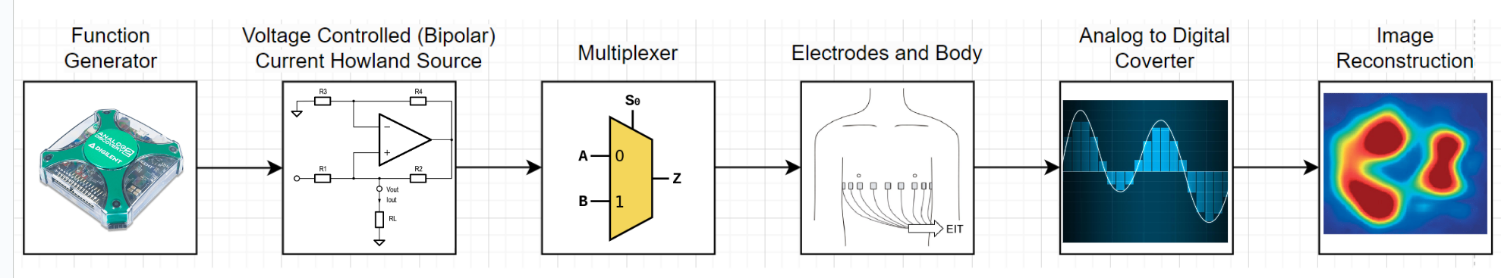
\includegraphics[width=6.83087in,height=1.26656in]{media/image4.png}

\subsection{DETAILED DESCRIPTION}\label{detailed-description}

\subsubsection{SYSTEM/COMPONENT 1 - Control}\label{systemcomponent-1---control}

The control system circuit consists of two 16:1 multiplexor (MUX) ICs.
The specific component used in the design was the ADG406BNZ, from Analog
Devices Inc. These MUXs are designed to direct 16 different signals to
or from one destination or source. The MUXs are being used to direct a
current from a respective Howland current source to one of 16
electrodes. The 16 MUX outputs connect the 16 electrodes with the NI
Boards read channels and are directed by 4 digital control signals.
Connecting each output of the MUXs will halve the amount of wire needed
and will not be an issue because the MUXs will not have the same
channels, permitting current flow at the same time. A single 12 V supply
will power the MUXs. A simple diagram of the control circuit is shown in
Figure 3.

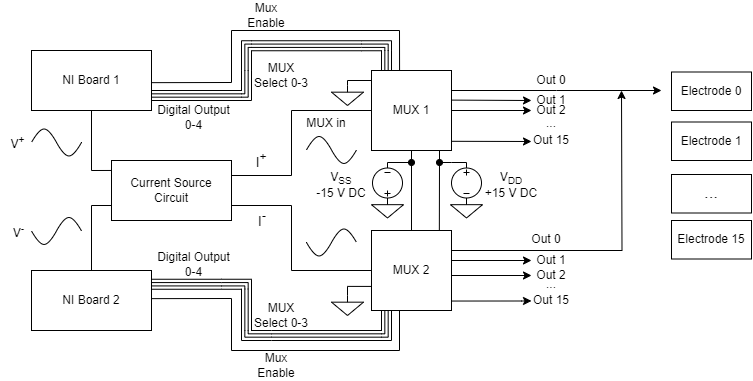
\includegraphics[width=6.5in,height=3.28889in]{media/image5.png}

\subsubsection{SYSTEM/COMPONENT 2 -- Current Injection}\label{systemcomponent-2-current-injection}

The current injection system consists of a multifrequency bipolar
signal. The signal contains a 10k, 25k, and 50k Hz signal with a peak
current of 10mA. The signals will be generated using the NI boards 180
degrees out of phase. The signal will then be sent through the Howland
current source where the current is restricted. The body has a varying
impedance as the patient breathes and the Howland current source keeps a
constant current output while impedance varies. Figure 4 below shows
both sides of a completed current source circuit.

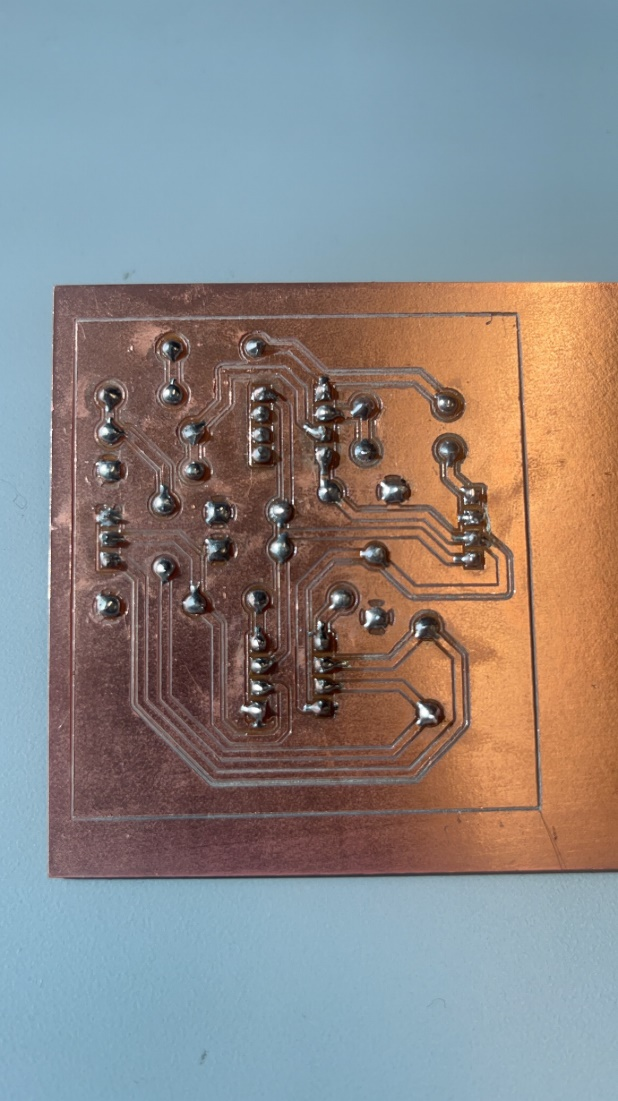
\includegraphics[width=2.56253in,height=2.30215in]{media/image6.jpeg}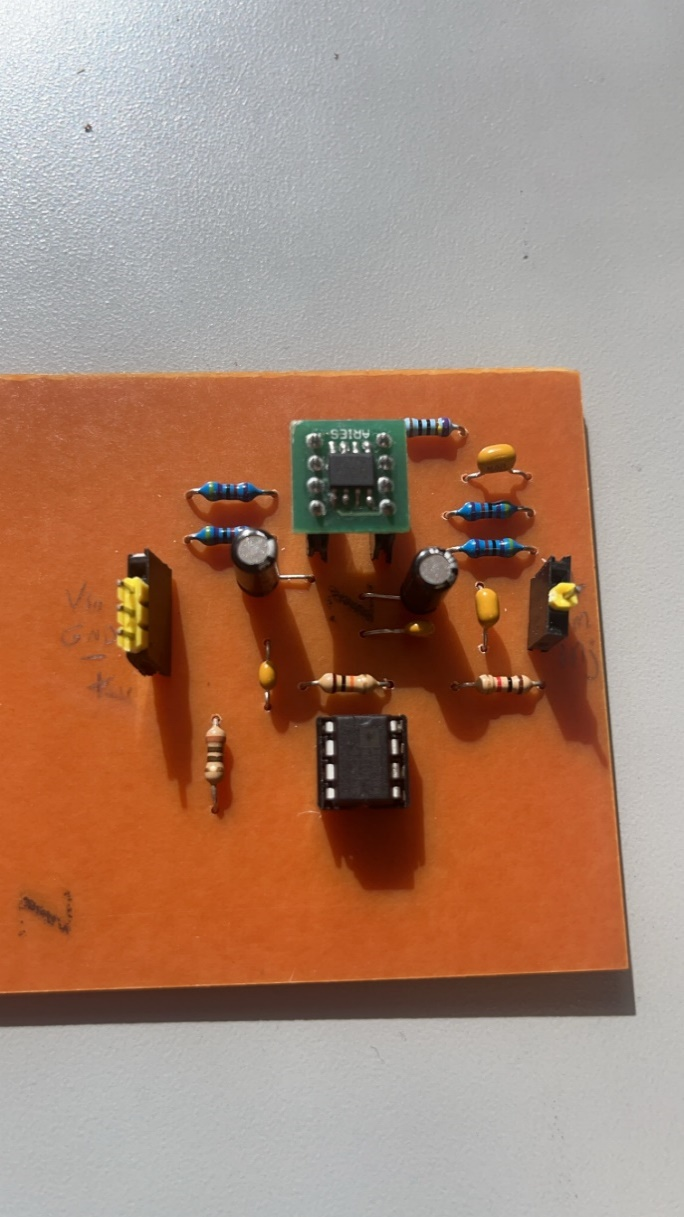
\includegraphics[width=2.6386in,height=2.29158in]{media/image7.jpeg}

\subsubsection{SYSTEM/COMPONENT 3 - Measurement}\label{systemcomponent-3---measurement}

The measurement system consists of 16 electrodes and two NI boards. The
NI boards read analog voltage signals from electrodes, which pick up
voltages created by the current injection system. The electrodes have
buffers that isolate the patient from the NI board and the current
directed by the MUX control circuit. The voltages read by the NI board
are then processed by a program written in MATLAB to create with code
supplied by Dr. Santos to create a real-time image. Figure 5 below shows
a simple layout of the active electrode circuit.

\includegraphics{media/image8.png}

\subsubsection{SYSTEM/COMPONENT 4 -- Power Supply}\label{systemcomponent-4-power-supply}


The power supply system provides power to all the IC components; each
requiring a different voltage. The first component running from a 60Hz,
120 V, standard AC wall outlet is a 120 V AC to 24 V DC converter.
Following this converter is multiple DC to DC converters. A 24 V DC to
plus and minus 15 V DC converter is used to provide power to the two
MUXs of the control circuit and provide power for the current source
circuit.

\subsection{USE}\label{use}

To be completed Later

\section{Evaluation}\label{evaluation}

\subsection{Overview}\label{overview-1}

The test plan for the EIT machine requires testing on many components.
To be confirmed was that two three-frequency voltage signals, consisting
of 10, 30, and 50 kHz, 180 degrees out of phase, were produced by the NI
board that was to be then converted into a current signal that was not
to exceed 10 mA, with a 1\% margin of error for accuracy. This current
signal delivery system was tested for accuracy and consistency with
voltage measurements by taking voltage measurements with an oscilloscope
over a resister.

A control system was also tested to ensure that timing and current
direction would be delivered to the appropriate electrodes at the
appropriate time. Testing of the control system was done by measuring
voltage signals at the electrodes while stepping through the control
system slowly while ensuring that the proper electrode was receiving the
signal. The control system was also to implement the skip-four pattern
of current injection.

The voltages produced on the electrodes were then to be read back in by
the ADC of the NI boards to processed by a MATLAB script. Ideally this
was to be done over 32 electrodes, at a sample rate of 1 Ms/s, verified
by settings designated by the created MATLAB script. At each each phase
of measurement, a single state of electrode current injection was to
provide a sample size between 500 to 1024 samples, which was simply
verified by viewing variables in MATLAB. MATLAB was also to be used to
provide real-time imaging, which would be verified by viewing a
real-time image of an object easily confirmed by placing objects in a
saltwater tank. A signal extraction technique was used to extract only
the desired input frequencies called Quadrature Demodulation and was
tested greatly to ensure its accuracy.

Current into the system used to power all circuitry needed to be current
limited as well to ensure safety. This was done by simply using
adjustable DC voltage sources using a single Gw Instek GPP-3323 DC power
supply. All circuits were to be done on CNC milled PCBs, was shown to be
completed with physically created PCBs that were implemented into use on
the EIT machine.
\begin{center}
    Table 4.1.1. Contains base requirements for EIT system.\\
    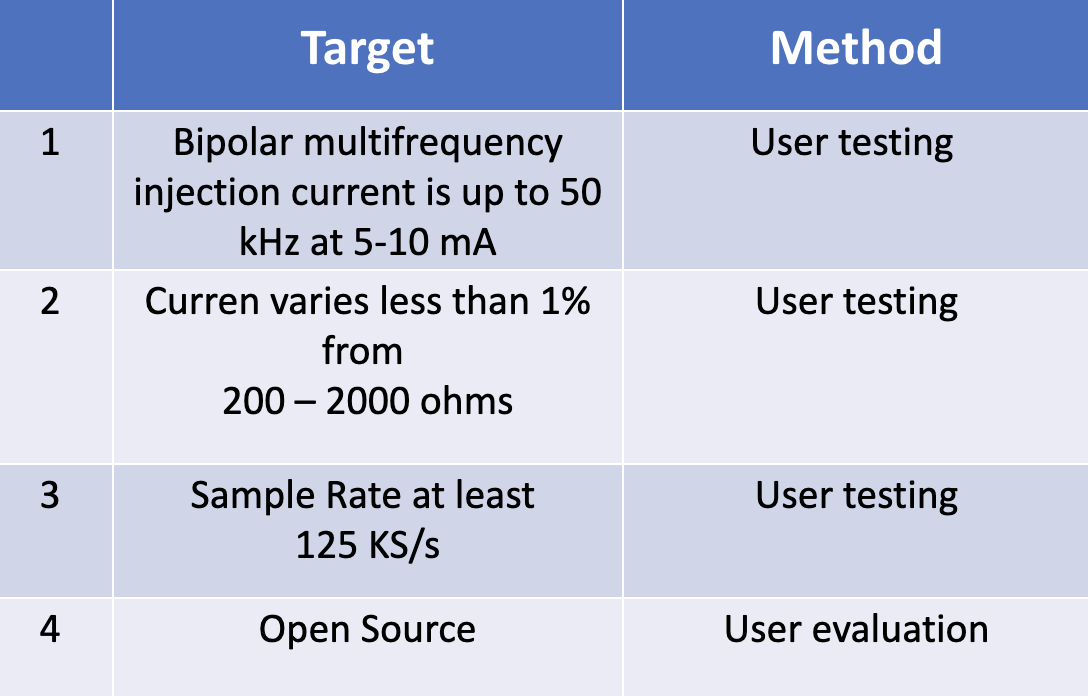
\includegraphics[width=4.59375in,height=2.94in]{media/image9.png}
\end{center}



\subsection{Evaluation of Howland Current Source Circuit and Signal Generation}\label{evaluation-of-howland-current-source-circuit-and-signal-generation}

\subsubsection{Purpose of Evaluation}\label{purpose-of-evaluation}

The signal sent to the patient must maintain a stable current across the
load resistance ranging from 500 to 2000 ohms. This requirement arises
from the fluctuating resistance within the patient\textquotesingle s
body, particularly during breathing cycles and lung inflation. It is
crucial to limit the deviation in current across these impedance ranges
to within 1\% to accurately capture the patient\textquotesingle s
impedance data, preventing distortion caused by signal artifacts. The
Howland current source employs DC-blocking capacitors at the signal
output to guarantee patient safety by preventing electric
shocks.

\subsubsection{4.2.2 Test Methods}\label{test-methods}

A single Howland circuit was tested with a variation of loads with an
input signal at the maximum frequency of 50kHz and a 6Vpp signal. This
expected approximately 7.75 mA output at 50kHz. This test allows the
current to be as high as possible without beginning to saturate.

\subsubsection{4.2.3 Results and Discussion}\label{results-and-discussion}

When the current surpasses 8mA at 1500 ohms, the output signal begins to
saturate due to the operational constraints of the Howlands AD8066 IC,
which is powered by +/- 12 volts and cannot exceed this output value. To
accommodate a resistance load of up to 2000 ohms, the design is limited
to utilizing up to 6 mA. Considering the system will be tested on a tank
with a resistance load of no more than 1500 Ohms, a current of 7.75 mA
is applied to optimize performance while avoiding saturation, as
indicated in Table 2. The table also displays an injection current error
within 6.4\%. Despite this proximity to the expected accuracy, it falls
short of the desired 1\% threshold set by our sponsor. Consequently, the
generated images may exhibit minor distortion if impedance fluctuates
between the minimum and maximum values.

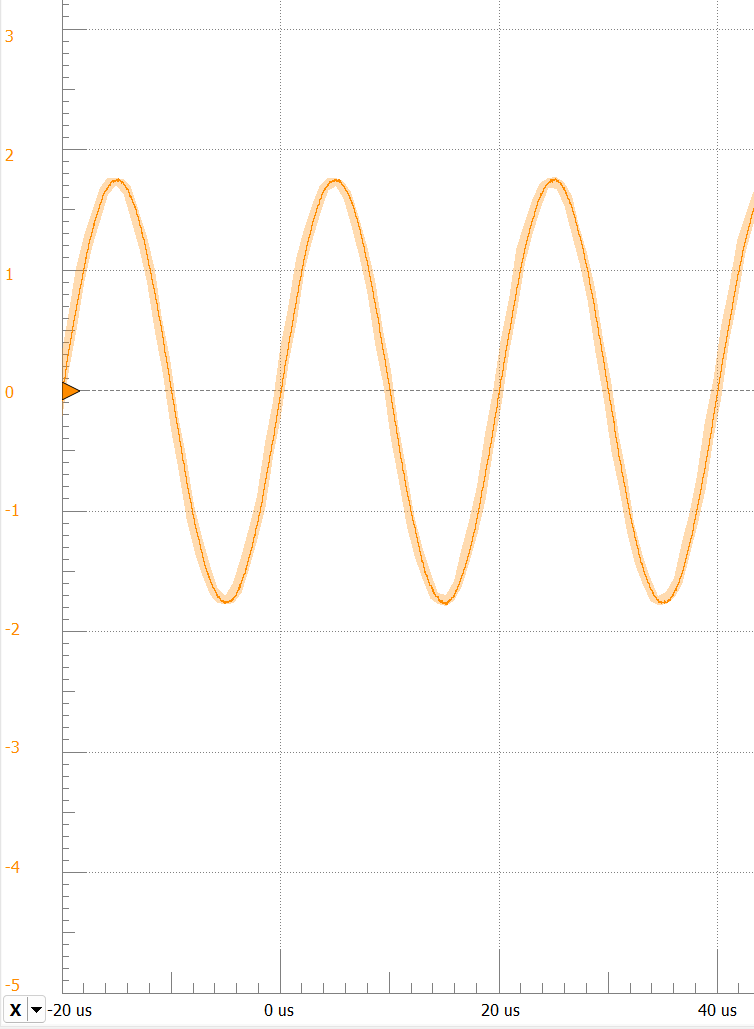
\includegraphics[width=4.61435in,height=4.23958in]{media/image10.png}

\end{document}